%-----------------------------------------------------------------------
% Beginning of chap2.tex
%-----------------------------------------------------------------------
%
%  AMS-LaTeX sample file for a chapter of a monograph, to be used with
%  an AMS monograph document class.  This is a data file input by
%  chapter.tex.
%
%  Use this file as a model for a chapter; DO NOT START BY removing its
%  contents and filling in your own text.
% 
%%%%%%%%%%%%%%%%%%%%%%%%%%%%%%%%%%%%%%%%%%%%%%%%%%%%%%%%%%%%%%%%%%%%%%%%


\chapter*{Lecture 7}
\addcontentsline{toc}{chapter}{Lecture 6}
\addtocounter{chapter}{7}
\addtocounter{section}{0}
%\numberwithin{section}{chapter}
\numberwithin{equation}{chapter}
\numberwithin{theorem}{chapter}

% \epigraph{}{--- \textup{}}
\epigraph{``[A]lmost every ``convex'' idea can be explained by a two-dimensional picture.''}{--- \textup{Alexander Barvinok}}

In this lecture we begin our study of the theory underlying constrained convex optimization. One way to define a {\em convex optimization problem} is
\begin{align*}
\begin{split}
 \minimize & f(\vct{x})\\
 \subjto & f_1(\vct{x})\leq 0\\
 & \cdots \\
 & f_m(\vct{x})\leq 0\\
 & \vct{x}\in \Omega
 \end{split}
\end{align*}
where $f,f_1,\dots,f_m\colon \R^n\to \R$ are {\em convex} functions and $\Omega\subseteq \R^n$ is a {\em convex} set. The special case where the $f$ and the $f_i$ are linear functions and $\Omega=\R^n$ is known as linear programming, and is studied first. Before embarking on the study of models and algorithms for convex optimization, we need to study convex sets in more depth.

\section{Convex sets}
We recall the definition of a convex set.
\begin{definition}
 A set $C\subseteq \R^n$ is a {\em convex set}, if for all $\vct{x},\vct{y}\in C$ and $\lambda\in [0,1]$, $\lambda\vct{x}+(1-\lambda)\vct{y}\in C$. In words, for every two points in $C$, the line joining them is also in $C$. A compact (closed and bounded) convex set is called a {\em convex body}.
\end{definition}

\begin{figure}[h!]
\centering
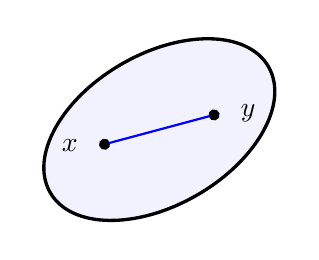
\begin{tikzpicture}[thick,rotate=15,scale=0.8]
\filldraw[color=black, fill=blue!5, very thick, rotate=15](0,0) ellipse (2 and 1.2);

\node (A1) at (-1,0)  [label=180:$\vct{x}$] {};
\node (A2) at (1,0)   [label=0:$\vct{y}$] {};
\filldraw[black] (-0.9,0) circle (2pt);
\filldraw[black] (0.9,0) circle (2pt);

\draw[color=blue,thick] (A1) -- (A2);
\end{tikzpicture}
\end{figure}

We will denote by $\mathcal{C}(\R^n)$ the collection of convex sets and by $\mathcal{K}(\R^n)$ the collection of convex bodies. The following Lemma is left as an exercise.

\begin{lemma}
 Let $C,D\in \mathcal{C}(\R^n)$ be convex sets. Then the following are also convex.
 \begin{itemize}
  \item $\displaystyle C\cap D$;
  \item $\displaystyle C+D=\{\vct{x}+\vct{y} \mid \vct{x}\in C, \vct{y}\in D\}$;
  \item $\displaystyle \mtx{A}C=\{\mtx{A}\vct{x} \mid \vct{x}\in C\}$, where $\mtx{A}\in \R^{m\times n}$.
 \end{itemize}
\end{lemma}

The {\em convex hull} $\conv{S}$ of a set $S$ is the intersection of all convex sets containing $S$. Clearly, if $S$ is convex, then $S=\conv{S}$.

\begin{example}
 Let $S=\{(1,1)^{\trans},(1,-1)^{\trans},(-1,1)^{\trans},(-1,-1)^{\trans},(0,0)^{\trans}\}$. The convex hull of this set is the square.
 \begin{figure}[h!]
\centering
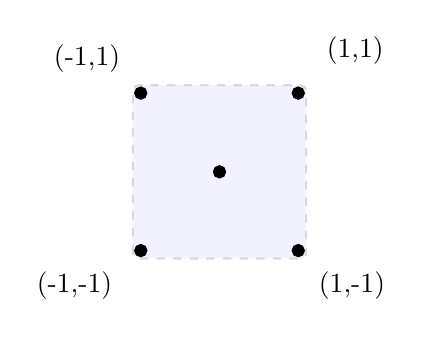
\begin{tikzpicture}[thick,scale=1]
\node (A1) at (-1.1,-1.1)  [label=195:{(-1,-1)}] {};
\node (A2) at (1.1,1.1)   [label=45:{(1,1)}] {};
\node (A3) at (-1,1)  [label=135:{(-1,1)}] {};
\node (A4) at (1,-1)   [label=-45:{(1,-1)}] {};
\node (A5) at (0,0)   [label=90:{(0,0)}] {};
\draw[color=black!15, fill=blue!5, thick, rounded corners=2pt, dashed] (A1) rectangle (A2);
\filldraw[black] (1,1) circle (2pt);
\filldraw[black] (1,-1) circle (2pt);
\filldraw[black] (-1,1) circle (2pt);
\filldraw[black] (-1,-1) circle (2pt);
\filldraw[black] (0,0) circle (2pt);
\end{tikzpicture}
\caption{A convex hull of five points.}
\end{figure}
\end{example}

A {\em convex combination} of points $\vct{x}_1,\dots,\vct{x}_k$ is a linear combination
\begin{equation*}
 \sum_{i=1}^k \lambda_i \vct{x}_i
\end{equation*}
such that $\lambda_i\geq 0$ and $\sum_{i=1}^k \lambda_i = 1$. It can be shown inductively that convex sets are closed under convex combinations: any convex combination of points in $C\in \mathcal{C}(\R^n)$ is still in $C$. In fact, the set of all convex combinations of points in a set $S$ is the convex hull of $S$.

\begin{lemma}
 Let $S$ be a set. Then 
 \begin{equation*}
  \conv{S} = \{\vct{x}\in \R^n \mid \vct{x}=\sum_{i=1}^k \lambda_i \vct{x}_k, \ \vct{x}_i\in S, \ \sum_{i=1}^k \lambda_i = 1, \ \lambda_i\geq 0\}.
 \end{equation*}
\end{lemma}

\begin{example}
A hyperplane, defined as the solution set of one linear equation,
\begin{equation*}
 H = \{\vct{x} \mid \ip{\vct{a}}{\vct{x}} = b\},
\end{equation*}
is a convex set.
Define the halfspaces $H_+$ and $H_-$ as the two sides that $H$ divides $\R^n$ into:
\begin{equation*}
 H_- = \{\vct{x}\mid \ip{\vct{a}}{\vct{x}}\leq b\}, \quad H_+ = \{\vct{x}\mid \ip{\vct{a}}{\vct{x}}\geq b\}
\end{equation*}
These are also convex sets. 
\begin{figure}[h!]
\centering
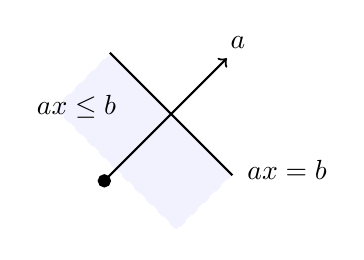
\begin{tikzpicture}[thick,rotate=-45]
\coordinate (A1) at (-1.1,0);
\coordinate (A2) at (1.1,0);
\coordinate (A3) at (0,-1.2);
\coordinate (A4) at (0,1);
\coordinate (A5) at (1.1,-1);

\draw[color=black!0, fill=blue!5, thick, dashed] (A1) rectangle (A5);
\draw[color=black, thick] (A1) -- (A2);
\draw[color=black, thick,->] (A3) -- (A4);
\filldraw[black] (A3) circle (2pt);

\node (A) at (0.2,1) [label=90:$\vct{a}$] {};
\node (H) at (1,0) [label=0:{$\ip{\vct{a}}{\vct{x}}=b$}] {};
\node (Hm) at (-1.2,-0.5) [label=270:{$\ip{\vct{a}}{\vct{x}}\leq b$}] {};
\end{tikzpicture}
\caption{Hyperplane and halfspace}
\end{figure}
\end{example}

\begin{example}
 Euclidean balls and ellipsoids are common examples of convex sets. Let $\mtx{P}$ be a positive semidefinite symmetric matrix. Then an ellipsoid with center $\vct{x}_0$ is a set of the form
 \begin{equation*}
  \mathcal{E} = \{\vct{x} \mid \ip{\vct{x}-\vct{x}_0}{\mtx{P}^{-1}(\vct{x}-\vct{x}_0)}\leq 1\}.
 \end{equation*}
A Euclidean unit ball is the special case $\mtx{P}=\mtx{I}$.
\begin{figure}[h!]
\centering
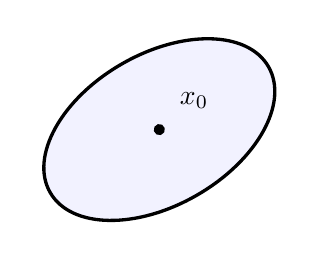
\begin{tikzpicture}[thick,rotate=15,scale=0.8]
\filldraw[color=black, fill=blue!5, very thick, rotate=15](0,0) ellipse (2 and 1.2);

\node (A1) at (0,0)  [label=45:{$\vct{x}_0$}] {};
\filldraw[black] (0,0) circle (2pt);
\end{tikzpicture}
\caption{An ellipse}
\end{figure}
\end{example}

\begin{example}
 A {\em convex cone} is a set $C$ such that for all $\vct{x},\vct{y}$ and $\lambda\geq 0, \mu\geq 0$,
 $\lambda \vct{x}+\mu \vct{y}\in C$. It is easily verified that such a set is convex. Three important cones are the following:
 \begin{enumerate}
  \item The non-negative orthant $\R^n_{+}=\{\vct{x}\in \R^n \mid x_i\geq 0, 1\leq i\leq n\}$,
  \item The second order (ice cream) cone (or Lorentz cone)
  \begin{equation*}
   C_{\alpha} = \{\vct{x} \mid \sum_{i=1}^{n-1}x_i^2\leq x_n^2\},
  \end{equation*}
  \item The cone $\mathcal{S}_{+}^n$ of positive semidefinite symmetric matrices.
 \end{enumerate}
\begin{figure}[h!]
\centering
 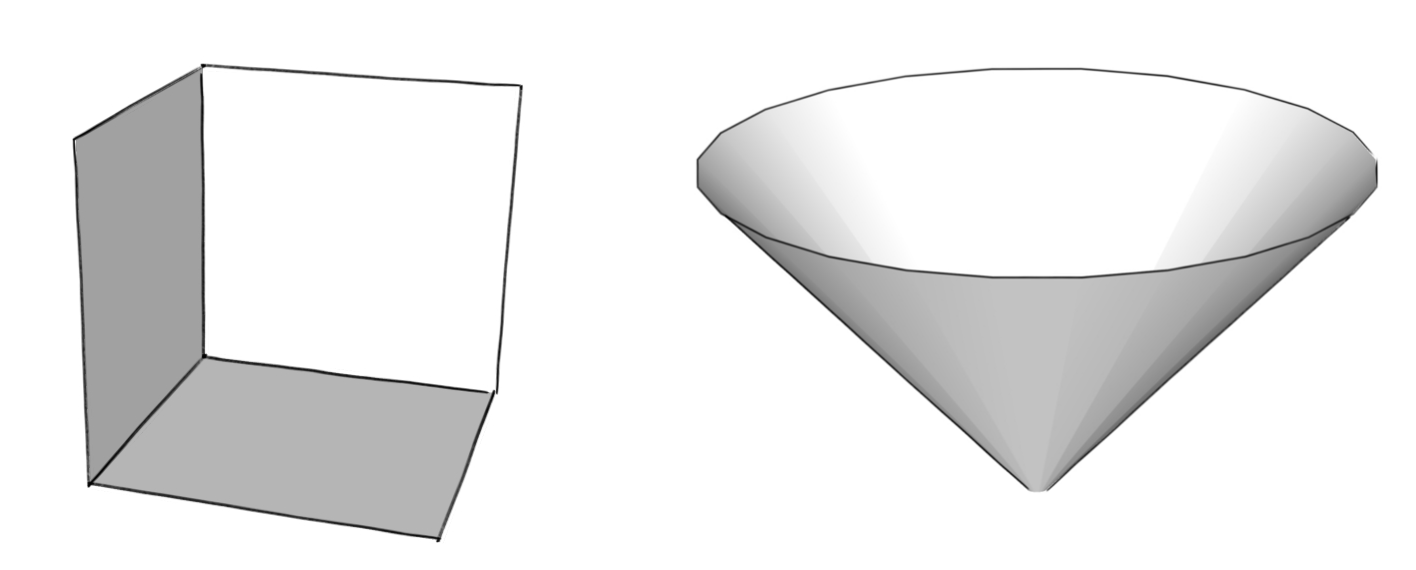
\includegraphics[width=0.6\textwidth]{images/cones.png}
 \caption{The orthant and the second order cone}
\end{figure}

\end{example}


Possibly the most important result in convex geometry is the {\em hyperplane separation theorem}.  We first need the following.

\begin{lemma}\label{le:obtuse}
 Let $C$ be a non-empty convex set and $\vct{x}\not\in C$. Then there exists a point $\vct{y}\in C$ that minimizes the distance $\norm{\vct{x}-\vct{y}}$. Moreover, for all $\vct{z}\in C$ we have
 \begin{equation*}
  \ip{\vct{z}-\vct{y}}{\vct{x}-\vct{y}}\leq 0.
 \end{equation*}
In words, the vectors $\vct{z}-\vct{y}$ and $\vct{x}-\vct{y}$ form an obtuse angle.
\end{lemma}

\begin{figure}[h!]
\centering
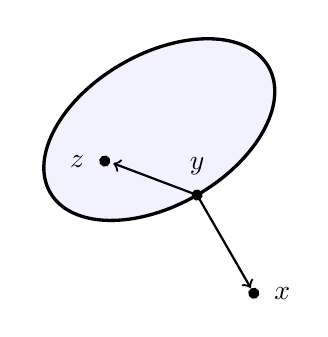
\begin{tikzpicture}[thick,rotate=30,scale=0.8]
\filldraw[color=black, fill=blue!5, very thick](0,0) ellipse (2 and 1.2);
\node (A1) at (0,-3)  [label=0:{$\vct{x}$}] {};
\node (A2) at (0,-1.2)  [label=90:{$\vct{y}$}] {};
%\node (A3) at (0,-2.5)  [label=180:{$\vct{a}$}] {};
\node (A4) at (-1,0)  [label=180:{$\vct{z}$}] {};
\filldraw[black] (0,-3) circle (2pt);
\filldraw[black] (0,-1.2) circle (2pt);
\filldraw[black] (-1,0) circle (2pt);
\draw[color=black, thick, <-] (0,-2.9) -- (0,-1.2);
\draw[color=black, thick, <-] (-0.9,-0.1) -- (0,-1.2);
\end{tikzpicture}
\caption{Internal and external directions} \label{fig:neg}
\end{figure}

\begin{proof}
 Since $C\neq \emptyset$, there exists $r>0$ such that the ball $B(\vct{x},r):=\{\vct{y}\in \R^n \mid \norm{\vct{y}-\vct{x}}\leq \e\}$ intersected with $C$ is not empty. Since $K:=C\cap B(\vct{x},r)$ is compact (closed and bounded) and the function $\norm{\vct{y}-\vct{x}}$ is continuous on $K$, it has a minimizer $\vct{y}\in K$. For the second claim, note that since $C$ is convex, for every $\lambda\in [0,1]$,
 \begin{equation*}
  \vct{w} = \lambda \vct{z}+(1-\lambda)\vct{y} \in C.
 \end{equation*}
For the distance between $\vct{z}$ and $\vct{x}$ we then get
\begin{align*}
 \norm{\vct{w}-\vct{x}}^2  &= \norm{\lambda\vct{z}+(1-\lambda) \vct{y}-\vct{x}}^2 = \norm{\lambda (\vct{z}-\vct{y})-(\vct{x}-\vct{y})}^2\\
 &= \lambda^2\norm{\vct{z}-\vct{y}}^2-2\lambda \ip{\vct{z}-\vct{y}}{\vct{x}-\vct{y}}+\norm{\vct{x}-\vct{y}}^2.
\end{align*}
We now prove the claim by contradition. Assume $\ip{\vct{z}-\vct{y}}{\vct{x}-\vct{y}}>0$. Then we can choose $\lambda$ such that
\begin{equation*}
 0< \lambda < \min\left\{ \frac{2\ip{\vct{x}-\vct{y}}{\vct{z}-\vct{y}}}{\norm{\vct{z}-\vct{y}}^2} , 1\right\}.
\end{equation*}
With such a $\lambda$ we get
\begin{equation*}
 \norm{\vct{w}-\vct{x}}^2 = \lambda^2\norm{\vct{z}-\vct{y}}^2-2\lambda \ip{\vct{z}-\vct{y}}{\vct{x}-\vct{y}}+\norm{\vct{x}-\vct{y}}^2 < \norm{\vct{x}-\vct{y}}^2.
\end{equation*}
This inequality, however, contradicts the assumption that $\vct{y}$ is a closest point, so that
$\ip{\vct{z}-\vct{y}}{\vct{x}-\vct{y}}\leq 0$ has to hold.
\end{proof}

In what follows write $\inter S$ for the {\em interior} of a set $S$.

\begin{theorem}
 Let $C$ be a closed convex set and $\vct{x}\not\in C$. Then there exists a hyperplane $H$ such that $C\subset \inter H_-$ and $\vct{x}\in \inter H_+$. 
\end{theorem}

\begin{figure}[h!]
\centering
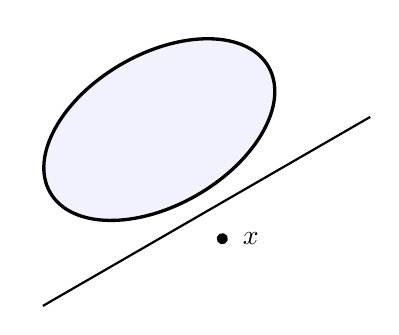
\begin{tikzpicture}[thick,rotate=30,scale=0.8]
\filldraw[color=black, fill=blue!5, very thick](0,0) ellipse (2 and 1.2);

\node (A1) at (0,-2)  [label=0:{$\vct{x}$}] {};
\filldraw[black] (0,-2) circle (2pt);
\draw[color=black, thick] (-3,-1.5) -- (3,-1.5);
\end{tikzpicture}
\caption{A separating hyperplane}
\end{figure}

\begin{proof}
 Let $\vct{y}\in C$ be a nearest point to $\vct{x}$ in $C$, i.e., a point such that for all other $\vct{z}\in C$, $\norm{\vct{x}-\vct{y}}\leq \norm{\vct{x}-\vct{z}}$. Define
 \begin{equation*}
  \vct{a}= \vct{x}-\vct{y}, \quad b = (\norm{\vct{x}}^2-\norm{\vct{y}}^2)/2.
 \end{equation*}
We aim to show that $\ip{\vct{a}}{\vct{x}} = b$ defines a separating hyperplane. 

For this we have to show that
\begin{enumerate}
 \item $\ip{\vct{a}}{\vct{x}}>b$;
 \item For all $\vct{z}\in C$, $\ip{\vct{a}}{\vct{z}}<b$.
\end{enumerate}
For (1), note that 
\begin{equation*}
 \ip{\vct{a}}{\vct{x}} = \ip{\vct{x}-\vct{y}}{\vct{x}}>\ip{\vct{x}-\vct{y}}{\vct{x}}-\frac{1}{2}\norm{\vct{x}-\vct{y}}^2 = \frac{1}{2}(\norm{\vct{x}}^2-\norm{\vct{y}}^2) = b.
\end{equation*}
To prove (2), assume on the contrary that there exists a $\vct{z}\in C$ such that $\ip{\vct{a}}{\vct{z}}\geq b$. We know that the point $\vct{y}\in C$ satisfies the inequality (2), since
\begin{equation*}
 \ip{\vct{a}}{\vct{y}} < \ip{\vct{a}}{\vct{y}}+\frac{1}{2}\norm{\vct{a}}^2 = \ip{\vct{a}}{\vct{y}}+\frac{1}{2}\norm{\vct{x}-\vct{y}}^2 = b.
\end{equation*}
Therefore, 
\begin{equation*}
 \ip{\vct{a}}{\vct{z}-\vct{y}} = \ip{\vct{a}}{\vct{z}}-\ip{\vct{a}}{\vct{y}} > b-b = 0,
\end{equation*}
but this contradicts Lemma~\ref{le:obtuse}. We therefore conclude $\ip{\vct{a}}{\vct{z}}<b$. The separating hyperplane $H$ is thus defined by the equation $\ip{\vct{a}}{\vct{x}}=b$. 
\end{proof}

% %-----------------------------------------------------------------------
% % End of chap1.tex
% %-----------------------------------------------------------------------
